% Submission draft in the section structure of AGU journals (Global Biogeochemical Cycles).
% Generated by build.py from paper/MANUSCRIPT.md; edit the Markdown sources, not main.tex.
% For submission, move the content into AGU's agujournal2019 class (Overleaf "AGU Journal Template").
\documentclass[11pt]{article}
\usepackage[a4paper,margin=2.5cm]{geometry}
\usepackage{fontspec}
\setmainfont{STIXGeneral}
\usepackage{unicode-math}
\setmathfont{STIX Two Math}
\usepackage{graphicx,longtable,booktabs,array,calc,amsmath}
\usepackage[authoryear,round]{natbib}
\usepackage[hidelinks]{hyperref}
\usepackage{lineno,setspace}
\linenumbers
\onehalfspacing
\providecommand{\tightlist}{\setlength{\itemsep}{0pt}\setlength{\parskip}{0pt}}
\makeatletter
\def\fps@figure{tbp}
\makeatother
\setcounter{secnumdepth}{2}

\title{Upper-ocean carbon accumulates 16--18\,\% faster than tracer-based anthropogenic CO$_2$ estimates predict: a drift-immune, sample-matched test against fifty years of GLODAP DIC}
\author{Ishaan Sodhi\\[2pt]\small [Affiliation to be added]\\\small Corresponding author: [e-mail to be added]}
\date{Submission draft, \today}

\begin{document}
\maketitle

\section*{Key Points}\label{key-points}
\addcontentsline{toc}{section}{Key Points}

\begin{itemize}
\tightlist
\item
  One estimator applied to observed DIC and tracer-based anthropogenic
  carbon at 342,277 GLODAP samples, with cruise offsets and drift
  removed
\item
  Upper-ocean DIC accumulates 16--18 \% faster than TRACE predicts,
  consistently across basins and matched by two eMLR(C*) products
\item
  An Earth system model sampled like GLODAP shows the same TRACE
  shortfall, mostly from its damped surface CO\textsubscript{2} boundary
  condition
\end{itemize}

\section*{Abstract}\label{abstract}
\addcontentsline{toc}{section}{Abstract}

Anthropogenic CO\textsubscript{2} (C\textsubscript{ant}) in the ocean
interior is inferred either from repeated measurements of dissolved
inorganic carbon (DIC) or from transient-tracer age distributions, and
the two are usually compared only as gridded inventories. We apply one
within-location estimator to observed DIC and to tracer-based
C\textsubscript{ant} from TRACE at the same 342,277 GLODAPv2.2023
samples (1972--2021), conditioning on potential temperature, salinity
and apparent oxygen utilisation. A differential estimator with cruise
fixed effects is immune to any additive per-cruise offset, including
offsets that drift with time. In the upper ocean (γ\textsuperscript{n} ≤
27.0 kg m\textsuperscript{−3}), DIC accumulated 16 \% {[}11--21 \%{]}
faster than TRACE predicts, and 18 \% {[}11--23 \%{]} faster relative to
the deep ocean once cruise offsets are removed. The excess is similar in
all four basins, is matched at the same samples by two eMLR(C*) products
(13--20 \%), and is not explained by uniform scale drift or by the
choice of reference layers. In an Earth system model sampled at the same
points, the estimators recover the model's exact C\textsubscript{ant}
rate, and TRACE falls 12 \% short of it. Replacing TRACE's damped
surface CO\textsubscript{2} boundary condition by the atmospheric record
removes about 60 \% of the observed excess and most of the model
shortfall. The deep Atlantic, by contrast, accumulates 25--35 \% less
carbon than the steady-state expectation. These results provide a
drift-immune observational constraint on tracer-based
C\textsubscript{ant} accumulation rates.

\section*{Plain Language Summary}\label{plain-language-summary}
\addcontentsline{toc}{section}{Plain Language Summary}

The ocean absorbs a large share of the carbon dioxide released by human
activity. Because this extra carbon cannot be measured separately from
the carbon naturally present in seawater, scientists estimate it in two
ways: from repeated carbon measurements, or from the ``age'' of water
derived from other chemical tracers. We compared the two directly,
sample by sample, over fifty years of ship-based measurements, using a
method that cannot be fooled by small calibration differences between
research cruises. In the upper ocean, carbon has built up 16--18 \%
faster than the tracer-based method predicts. A climate model, analysed
in exactly the same way, shows a similar gap, and most of it traces back
to how the tracer method represents carbon dioxide at the sea surface.
Correcting this would raise estimates of how fast the upper ocean is
storing human-made carbon.

\section{Introduction}\label{introduction}

The ocean has taken up roughly a quarter to a third of anthropogenic
CO\textsubscript{2} emissions. The interior storage of this
anthropogenic carbon (C\textsubscript{ant}) is the most direct
observational constraint on that sink
\citep{Sabine2004, Gruber2019, Mueller2023}. C\textsubscript{ant} is
chemically indistinguishable from natural dissolved inorganic carbon
(DIC), so it is inferred, never measured.

Two families of methods do this:

\begin{itemize}
\tightlist
\item
  \textbf{DIC-based methods} separate C\textsubscript{ant} from repeated
  DIC measurements using regressions on hydrographic properties: eMLR
  and eMLR(C*) \citep{Friis2005, ClementGruber2018, Carter2017}.
\item
  \textbf{Tracer-based methods} infer the age distribution of water from
  transient tracers and combine it with the atmospheric
  CO\textsubscript{2} history and an assumed surface boundary condition,
  under steady circulation. This is the transit-time-distribution (TTD)
  approach \citep[e.g.,][]{Steinfeldt2024}.
\end{itemize}

TRACE \citep{Carter2025, Sandborn2026} makes TTD-based
C\textsubscript{ant} available for any sample from its position,
temperature, salinity and date, and is not trained on DIC. Its
validation agrees ``satisfactorily'' with DIC-based estimates, but only
at the level of global and regional inventories \citep{Sandborn2026}.

Where the two families disagree, the disagreement is informative. It
points to a bias in one method, to a change in natural carbon, or to a
change in circulation that violates the steady-state assumption
\citep{Gruber2019, Mueller2023}. To our knowledge, no study has applied
one identical estimator to observed DIC and to TTD-predicted
C\textsubscript{ant} at the same samples over the full GLODAP record.
Doing so removes differences in sampling geometry, mapping and period
that confound inventory-level comparisons.

Such a comparison faces a practical obstacle. The signal is about 0.1
µmol kg\textsuperscript{−1} yr\textsuperscript{−1}, and residual
inter-cruise DIC offsets in GLODAP are up to about 4 µmol
kg\textsuperscript{−1} \citep{Olsen2016, Lauvset2024}. A slow
calibration drift across decades would be indistinguishable from a
trend. We therefore introduce an estimator that is immune to additive
cruise-level offsets, including offsets that drift with time.

This work grew out of an audit of an empirical-regression project that
modelled DIC as a static function of salinity, temperature and apparent
oxygen utilisation (AOU). Its temporal-holdout errors contained a
systematic, depth-structured drift, the signature of anthropogenic
carbon uptake. Here we make that signal the object of study and ask:

\begin{quote}
Within fixed locations and at fixed (θ, S, AOU), is the observed rate of
DIC change, by basin and neutral-density layer, consistent with the rate
of C\textsubscript{ant} accumulation predicted by TRACE at the same
samples, once measurement drift between cruises is controlled?
\end{quote}

\section{Data}\label{data}

\textbf{GLODAPv2.2023.} We use the merged master file
{[}\citet{Lauvset2024}; NOAA NCEI accession 0283442; SHA-256
\texttt{002881fa…8766}{]}. Strict quality control keeps samples with
WOCE flag 2 and secondary-QC flag 1 for DIC, salinity and oxygen, plus
finite θ, pressure and neutral density γⁿ (428,264 samples). A relaxed,
range-only QC (512,384 samples) serves as an ablation.

\textbf{Domain.} The study covers the Atlantic, Indian and Pacific
(GLODAP regions 1, 16 and 8, north of 35°S) and the Southern Ocean
(south of 35°S); the Arctic is excluded. Samples are sorted into nine
neutral-density layers (edges γⁿ = 26.0, 26.5, 27.0, 27.5, 27.8, 28.0,
28.1, 28.2 kg m\textsuperscript{−3}) and grouped in 4°×4° cells. Only
cells whose observations span at least 10 years enter the analysis.
After these rules, the analysis uses 342,277 samples from 515 cruises
(1972--2021), in 5,865 cell × layer units across 34 basin × layer groups
(Fig. 1).

\begin{figure}
\centering
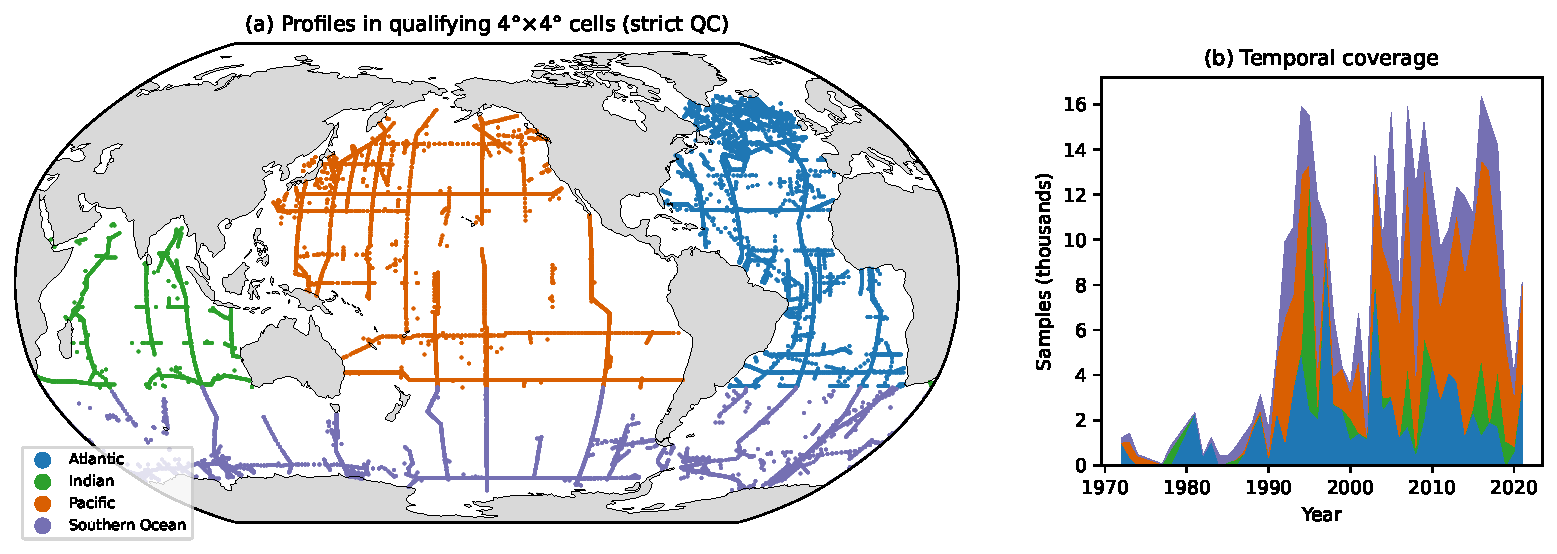
\includegraphics[width=1\linewidth,height=\textheight,keepaspectratio,alt={Study
data. (a) Positions of the profiles that enter the trend analysis:
strict-QC GLODAPv2.2023 samples in 4°×4° cells whose observations span ≥
10 years, coloured by basin. Robinson projection centred at 150°W. (b)
Number of these samples per year and basin
(thousands).}]{figures/fig1_study_area.pdf}
\caption{Study data. (a) Positions of the profiles that enter the trend
analysis: strict-QC GLODAPv2.2023 samples in 4°×4° cells whose
observations span ≥ 10 years, coloured by basin. Robinson projection
centred at 150°W. (b) Number of these samples per year and basin
(thousands).}
\end{figure}

\textbf{TRACE.} TRACE-Python v1.1.2 was evaluated at every sample with
the historical atmospheric trajectory and default settings. 400,755 of
402,747 strict-QC samples returned finite values. Seven structural
variants and an unadjusted surface boundary condition were also
evaluated (§3.4).

\textbf{Earth system model (E13).} MRI-ESM2-0 \citep{Yukimoto2019},
CMIP6 \citep{Eyring2016} \texttt{historical} r1i2p1f1 for 1972--2014 and
\texttt{ssp585} r1i2p1f1 for 2015--2021, on the regular 1° grid
(\texttt{gr}, version v20200303), read from the public Pangeo Google
Cloud copies. Variables:

\begin{itemize}
\tightlist
\item
  annual \texttt{dissic}, \texttt{dissicnat} and \texttt{o2};
\item
  monthly \texttt{thetao} and \texttt{so}, averaged to calendar years.
\end{itemize}

The model's exact anthropogenic carbon is
C\textsubscript{ant}\textsuperscript{true} = \texttt{dissic} −
\texttt{dissicnat} (natural DIC under pre-industrial atmospheric
CO\textsubscript{2}).

\textbf{eMLR(C*) products.} We use ΔC\textsubscript{ant} 1994--2007 of
\citet{Gruber2019} (NCEI 0186034; standard case and 14-member ensemble)
and ΔC\textsubscript{ant} 1994--2004 and 2004--2014 of
\citet{Mueller2023} (NCEI 0279447; standard case and 10 sensitivity
cases). Both are 1° gridded fields.

\section{Methods}\label{methods}

\subsection{Single-layer within-cell trend
(E02)}\label{single-layer-within-cell-trend-e02}

For each basin b and layer ℓ we fit

y\textsubscript{i} = α\_c(i) + f(θ\_i, S\textsubscript{i},
AOU\textsubscript{i}) + β·(t\textsubscript{i} − 2000) + ε\_i.

Here α\_c are cell fixed effects, f is a full quadratic in standardised
θ, S and AOU, and t is decimal year. The model is fitted by OLS after
within-cell demeaning. It is applied with y = observed DIC
(β\textsubscript{DIC}) and, at the same samples, with y = TRACE
C\textsubscript{ant} (β\textsubscript{Cant}), giving δ =
β\textsubscript{DIC} − β\textsubscript{Cant} and R =
β\textsubscript{DIC}/β\textsubscript{Cant}.

\subsection{Drift-immune differential trend
(E06)}\label{drift-immune-differential-trend-e06}

Any additive per-cruise offset that varies with time (calibration drift)
biases β one-for-one. To remove such offsets, each target layer ℓ (γⁿ ≤
27.8) is stacked with the deep reference layers (γⁿ \textgreater{} 27.8)
of the same basin, restricted to cruises that sampled both, and we fit

y\textsubscript{i} = α\_\{c×layer(i)\} + γ\textsubscript{cruise}(i) +
f\textsubscript{layer}(i)(θ\_i, S\textsubscript{i},
AOU\textsubscript{i}) + Δβ·(t\textsubscript{i} − 2000)·1{[}i ∈ ℓ{]} +
ε\_i.

The cruise effects γ absorb any additive offset of a cruise, whatever
its time dependence. Δβ is the trend of layer ℓ relative to the deep
reference, identified from within-cruise contrasts across cruises. We
solve the two-way fixed-effects system exactly: cell effects are swept
out, and cruise effects (≤ 300 per basin) enter through the Schur
complement of the normal equations. Applying the estimator identically
to DIC and C\textsubscript{ant} gives Δδ = Δβ\textsubscript{DIC} −
Δβ\textsubscript{Cant}.

The identifying assumption is that measurement offsets are additive and
depth-independent within a cruise. GLODAP's crossover-based secondary QC
rests on the same assumption. Δδ equals the absolute excess only if the
reference layers have none; we therefore report both δ (absolute,
drift-sensitive) and Δδ (relative, drift-immune).

\subsection{Uncertainty and pooling}\label{uncertainty-and-pooling}

Confidence intervals use a cruise-cluster bootstrap: cruises are
resampled with replacement and duplicate draws are kept (B = 300--500).
DIC and C\textsubscript{ant} are fitted jointly within each replicate.
For pooled statistics across layers and basins, one cruise resample per
replicate is shared by all groups, so pooled intervals are valid despite
shared cruises (E09, E11).

Synthetic tests calibrated both estimators:

\begin{itemize}
\tightlist
\item
  Single-layer estimator: random cruise offsets with SD 0--4 µmol
  kg\textsuperscript{−1} (E01).
\item
  Differential estimator: random offsets plus a linear drift of 0--0.1
  µmol kg\textsuperscript{−1} yr\textsuperscript{−1} (E06s).
\end{itemize}

\subsection{Sensitivity, controls and
comparators}\label{sensitivity-controls-and-comparators}

\begin{itemize}
\tightlist
\item
  \textbf{Analysis choices (Round 1):} relaxed QC; cell size 2°, 6° and
  8°; minimum span 5 and 15 years; linear conditioning; no AOU, no θ/S,
  or phosphate instead of AOU; post-1990 data only; seasonal harmonics;
  leave-one-cruise-out; no conditioning.
\item
  \textbf{TRACE structure (E07):} TTD shape Δ/Γ ∈ \{1.0, 1.6\} (default
  1.30); mean-age scale factors ×0.8 and ×1.2; air--sea disequilibrium
  scale ×0.9 and ×1.1; potential instead of in-situ temperature as
  input.
\item
  \textbf{Surface boundary condition (E12, post hoc):} TRACE's built-in
  surface CO\textsubscript{2} trajectory (``adjusted'') replaced by the
  atmospheric record.
\item
  \textbf{Pump-corrected response (E08):} C* = DIC −
  117·PO\textsubscript{4} − ½(TAlk + 16·PO\textsubscript{4})
  \citep{Gruber1996}, conditioned on θ and S only, on samples with
  measured, quality-controlled PO\textsubscript{4} and TAlk. The TAlk
  trend at fixed θ, S serves as a control variable.
\item
  \textbf{Time shape (E09b):} piecewise-linear trends with a knot at
  2000.
\item
  \textbf{eMLR(C*) products (E10):} C\textsubscript{ant} rate at the
  same samples and periods for both products and for TRACE, with no
  regression involved.
\item
  \textbf{Perfect-model test (E13):} MRI-ESM2-0 sampled at every
  sample's position, depth and year: nearest model column wet at that
  depth, linear in depth, unit conversion with in-situ density. AOU is
  computed from model O\textsubscript{2} and O\textsubscript{2}
  solubility at model θ, S. Basin, layer, cell, cruise and date
  assignments are the observed ones. Both estimators are applied to
  model θ, S, AOU and DIC, and compared with
  C\textsubscript{ant}\textsuperscript{true} and with TRACE run on model
  S and in-situ T. E13d (post hoc) repeats this with TRACE's unadjusted
  boundary condition.
\item
  \textbf{Alternative reference layers (E14):} the differential estimate
  (E11 form) with the reference restricted to γⁿ 27.8--28.0 or to γⁿ
  \textgreater{} 28.0.
\item
  \textbf{Near reference (E16):} the same estimate with the intermediate
  layers (27.0 \textless{} γⁿ ≤ 27.8) as reference and the 12 layers
  with γⁿ ≤ 27.0 as targets. This shortens the target--reference
  separation from kilometres to a few hundred metres, so an artefact
  that grows with depth or DIC contrast within a cruise would shrink the
  excess. E16b computes, for each layer, the uniform DIC scale drift
  that the single-layer and the differential excess would each require.
\end{itemize}

\subsection{Pre-registration}\label{pre-registration}

Round-1 hypotheses (H1--H4) and the Round-2 experiments E06--E10, with
their decision rules, were written down before computation
(\texttt{RESEARCH\_METHODOLOGY.md}, \texttt{GAP\_AUDIT\_ROUND2.md}). E11
(a summary of E06) and E12 were added after seeing the results and are
labelled post hoc throughout. In revision 3, E13 and E14 were
pre-registered (\texttt{GAP\_AUDIT\_ROUND3.md}) before any model data
were sampled. E13d was logged after seeing E13 and before running it.
E16 and E16b were pre-registered in \texttt{GAP\_AUDIT\_ROUND4.md}.

\subsection{Static empirical models}\label{static-empirical-models}

We re-implemented the original model hierarchy (mean, linear, rank-1,
rank-2, full-quadratic and cubic regressions of DIC on S, T and AOU).
Each was evaluated with and without a time or C\textsubscript{ant}
covariate under temporal, spatial-block and cruise-block validation.

\section{Results}\label{results}

\subsection{Both estimators recover known trends; only the differential
estimator survives
drift}\label{both-estimators-recover-known-trends-only-the-differential-estimator-survives-drift}

\begin{itemize}
\tightlist
\item
  \textbf{Single-layer estimator:} bias ≤ 0.012 µmol
  kg\textsuperscript{−1} yr\textsuperscript{−1} for trends of 0--1 µmol
  kg\textsuperscript{−1} yr\textsuperscript{−1}. Coverage of nominal 95
  \% intervals is about 91 \% under 4 µmol kg\textsuperscript{−1} cruise
  offsets (Fig. S1). Under a cruise-level drift d, its bias grows by
  exactly d.
\item
  \textbf{Differential estimator:} bias ≤ 0.002 µmol
  kg\textsuperscript{−1} yr\textsuperscript{−1} and coverage of 93--100
  \% for drifts of 0, 0.05 and 0.1 µmol kg\textsuperscript{−1}
  yr\textsuperscript{−1} (E06s).
\end{itemize}

\subsection{DIC rises at fixed properties with a ventilation
structure}\label{dic-rises-at-fixed-properties-with-a-ventilation-structure}

Observed DIC at fixed θ, S and AOU rises by about 1.0--1.1 µmol
kg\textsuperscript{−1} yr\textsuperscript{−1} in the lightest layers of
every basin, and the rate declines with density (Fig. 2). In the deep
layers:

\begin{figure}
\centering
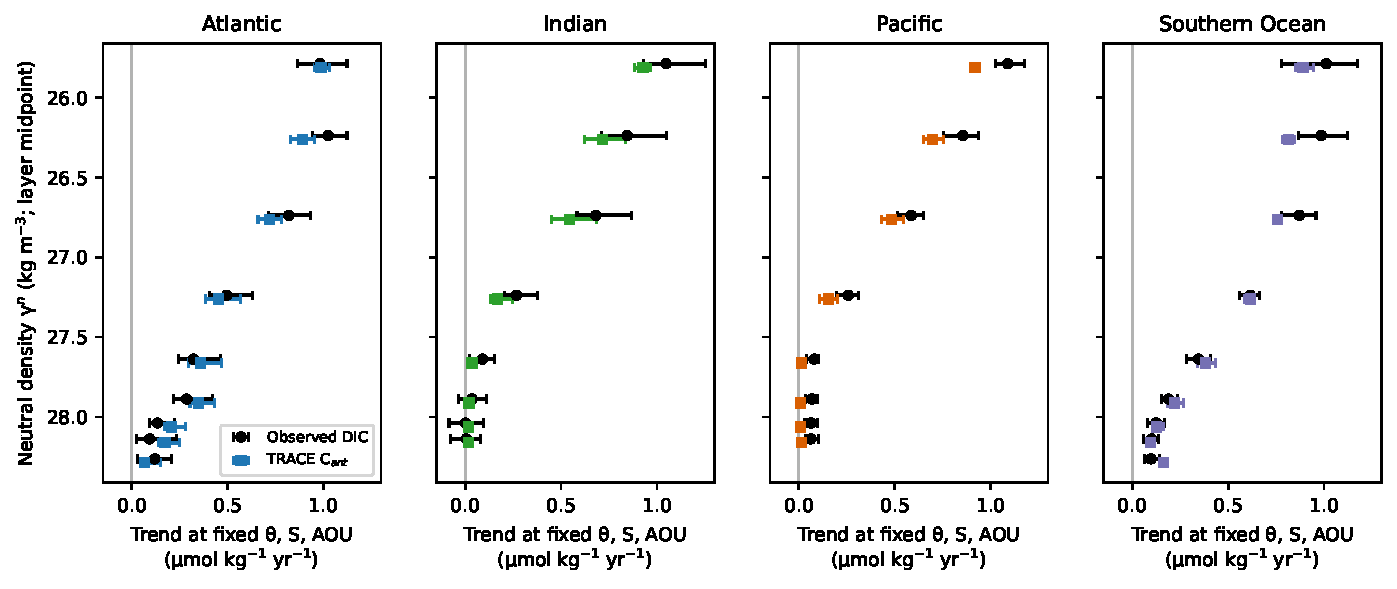
\includegraphics[width=1\linewidth,height=\textheight,keepaspectratio,alt={Rates
of change at fixed potential temperature, salinity and AOU (µmol kg−1
yr−1) by neutral-density layer. Layers are plotted at their midpoints;
the lightest is drawn at 25.6 and the densest at 28.35 kg m−3 for
display. Black circles: observed DIC (βDIC). Coloured squares: TRACE
Cant fitted with the identical estimator at the same samples (βCant).
Error bars: 95 \% cruise-cluster bootstrap intervals (B =
500).}]{figures/fig2_trend_profiles.pdf}
\caption{Rates of change at fixed potential temperature, salinity and
AOU (µmol kg\textsuperscript{−1} yr\textsuperscript{−1}) by
neutral-density layer. Layers are plotted at their midpoints; the
lightest is drawn at 25.6 and the densest at 28.35 kg
m\textsuperscript{−3} for display. Black circles: observed DIC
(β\textsubscript{DIC}). Coloured squares: TRACE C\textsubscript{ant}
fitted with the identical estimator at the same samples
(β\textsubscript{Cant}). Error bars: 95 \% cruise-cluster bootstrap
intervals (B = 500).}
\end{figure}

\begin{itemize}
\tightlist
\item
  Atlantic γⁿ 27.8--28.0 (North Atlantic Deep Water): 0.29 {[}0.22,
  0.42{]} µmol kg\textsuperscript{−1} yr\textsuperscript{−1}.
\item
  Deep Pacific: about 0.06.
\item
  Deep Indian Ocean: about 0.
\end{itemize}

The surface rate equals the equilibrium response of seawater to the
atmospheric CO\textsubscript{2} rise (≈ DIC/Revelle × d ln
pCO\textsubscript{2}/dt ≈ 1 µmol kg\textsuperscript{−1}
yr\textsuperscript{−1}).

\subsection{Observed DIC exceeds TRACE in the upper
ocean}\label{observed-dic-exceeds-trace-in-the-upper-ocean}

In 18 of 20 upper and intermediate layers, R is consistent with 1 within
TRACE's stated ±15 \% (H1; Fig. S2). Pooled over the 12 upper-ocean
groups (γⁿ ≤ 27.0) with a shared cruise bootstrap, however, observed DIC
rises faster than TRACE C\textsubscript{ant}: δ = 0.130 {[}0.090,
0.171{]} µmol kg\textsuperscript{−1} yr\textsuperscript{−1} and R = 1.16
{[}1.11, 1.21{]} (E09).

{\def\LTcaptype{none} % do not increment counter
\begin{longtable}[]{@{}ll@{}}
\toprule\noalign{}
Basin, upper ocean (γⁿ ≤ 27.0) & R {[}95 \% CI{]} \\
\midrule\noalign{}
\endhead
\bottomrule\noalign{}
\endlastfoot
Atlantic & 1.08 {[}1.02, 1.15{]} \\
Indian & 1.17 {[}1.07, 1.32{]} \\
Pacific & 1.19 {[}1.12, 1.28{]} \\
Southern Ocean & 1.16 {[}1.03, 1.26{]} \\
\end{longtable}
}

In intermediate layers the pooled excess is smaller (δ = 0.042 {[}0.019,
0.068{]}). In deep layers it is null overall (δ = −0.012 {[}−0.036,
0.013{]}), with basin-specific signs: Atlantic −0.065, Pacific +0.055.

\subsection{The excess is not caused by cruise-level calibration offsets
or
drift}\label{the-excess-is-not-caused-by-cruise-level-calibration-offsets-or-drift}

Because the deep Pacific and deep Atlantic deviations are depth-uniform
and of opposite sign, they are exactly what residual cruise offsets
would produce. The differential estimator removes them (Fig. 3).
Relative to the deep reference and with cruise effects absorbed:

\begin{figure}
\centering
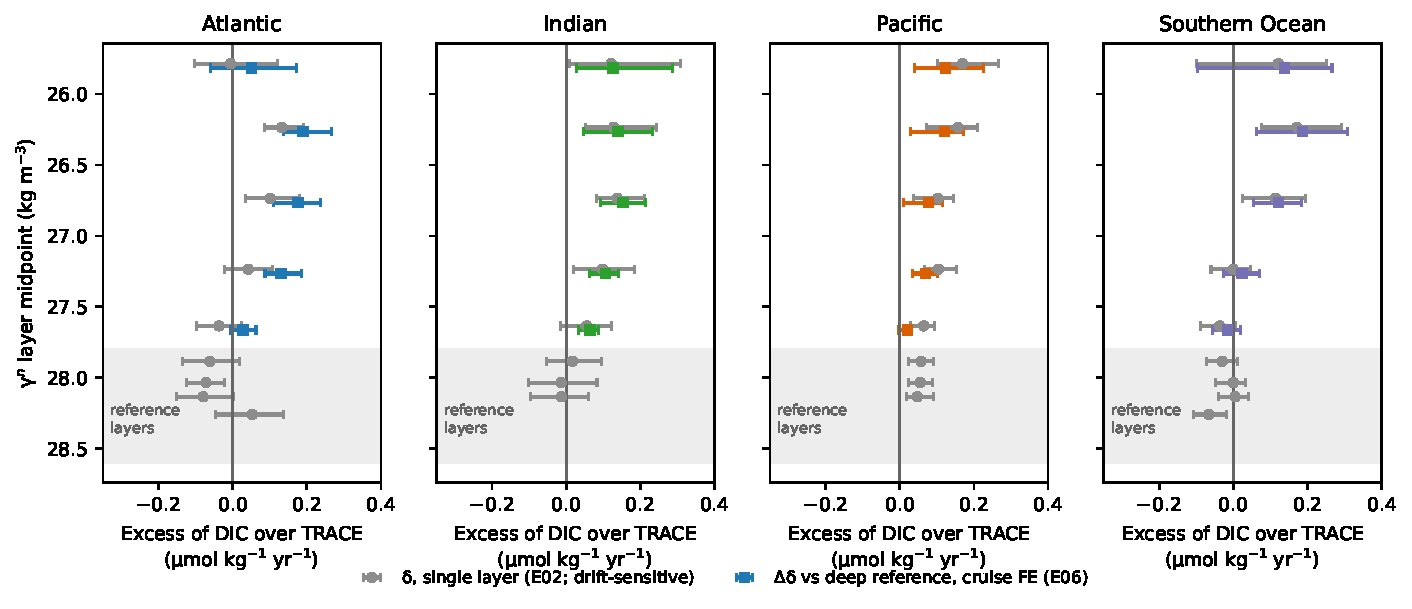
\includegraphics[width=1\linewidth,height=\textheight,keepaspectratio,alt={Excess
of DIC over TRACE (µmol kg−1 yr−1) by layer. Grey circles: single-layer
δ (E02), sensitive to cruise-level drift. Coloured squares: Δδ from the
differential estimator with cruise fixed effects (E06). It is relative
to the deep reference layers (grey shading, γⁿ \textgreater{} 27.8) and
immune to any additive per-cruise offset. Error bars: 95 \%
cruise-cluster bootstrap intervals (B =
300).}]{figures/fig7_drift_immune_excess.pdf}
\caption{Excess of DIC over TRACE (µmol kg\textsuperscript{−1}
yr\textsuperscript{−1}) by layer. Grey circles: single-layer δ (E02),
sensitive to cruise-level drift. Coloured squares: Δδ from the
differential estimator with cruise fixed effects (E06). It is relative
to the deep reference layers (grey shading, γⁿ \textgreater{} 27.8) and
immune to any additive per-cruise offset. Error bars: 95 \%
cruise-cluster bootstrap intervals (B = 300).}
\end{figure}

\begin{itemize}
\tightlist
\item
  Atlantic: Δδ = +0.19, +0.18, +0.13 (γⁿ 26.0--27.5).
\item
  Indian: +0.13 to +0.15 (γⁿ \textless{} 27.0).
\item
  Pacific: +0.12, +0.12, +0.08 (γⁿ \textless{} 27.0).
\item
  Southern Ocean: +0.19, +0.12 (γⁿ 26.0--27.0).
\end{itemize}

By the pre-registered rule, 10 of 12 upper layers show an ``excess not
explained by cruise offsets''. The other 2 are the sparsely sampled
Atlantic and Southern Ocean surface layers (γⁿ \textless{} 26), which
are inconclusive.

The Pacific single-layer excess shrinks by 0.03--0.05 under this
control, consistent with a small basin-wide offset. The Atlantic Δδ is
larger than δ because the Atlantic reference layers themselves
accumulate less than TRACE predicts (§4.8). The absolute upper-ocean
excess therefore lies between the E02 and E06 estimates in each basin,
and both are positive.

Cruise effects do not absorb an artefact that differs between upper and
deep samples within a cruise, for example a calibration error
proportional to DIC. Two pre-registered checks address this (E16):

\begin{itemize}
\tightlist
\item
  \textbf{Uniform scale drift is excluded.} For a uniform scale drift κ,
  the single-layer excess requires κ \textgreater{} 0. The differential
  excess requires κ \textless{} 0, because upper-ocean DIC is lower than
  deep DIC. The signs conflict in 11 of 12 upper layers. The
  differential excess alone would require a scale drift of 2--23 \% over
  50 years, far beyond the ≈ 0.1 \% accuracy of CRM-calibrated DIC.
\item
  \textbf{A near reference keeps most of the excess.} With the reference
  moved from the deep ocean to the intermediate layers (27.0 \textless{}
  γⁿ ≤ 27.8), the upper-ocean scale factor is m = 0.13 {[}0.06, 0.20{]},
  against 0.18 {[}0.11, 0.23{]} with the deep reference. This meets the
  pre-registered rule (CI excludes 0; within 0.08). The 30 \% reduction
  is within the uncertainty. It may reflect a smaller proportional
  excess in intermediate waters (§4.5) or a minor separation-dependent
  component.
\end{itemize}

\subsection{The excess is proportional to the TRACE
rate}\label{the-excess-is-proportional-to-the-trace-rate}

Across all 20 differential estimates, Δδ scales with the TRACE rate
(Fig. 4). The least-squares proportionality factor is m = 0.18 {[}0.11,
0.23{]} (E11, post hoc) and is similar in every basin:

\begin{figure}
\centering
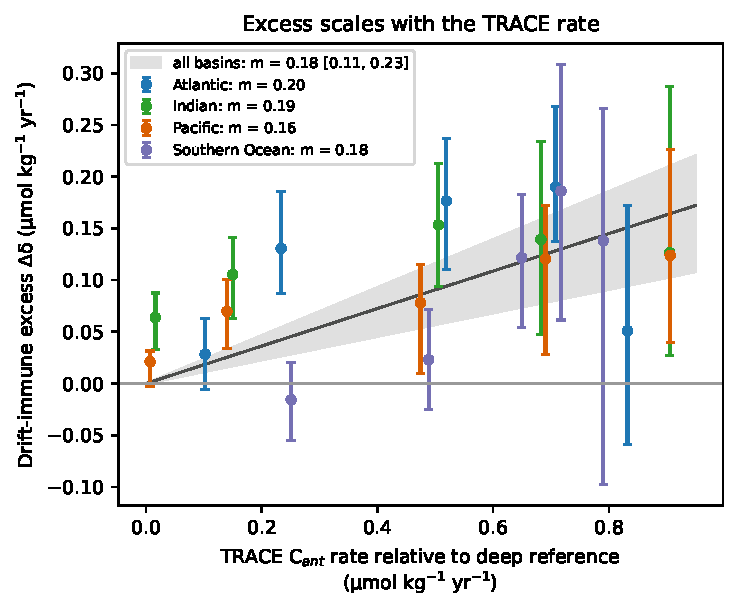
\includegraphics[width=1\linewidth,height=\textheight,keepaspectratio,alt={Drift-immune
excess Δδ versus the TRACE differential rate for the 20 upper and
intermediate basin × layer units, with 95 \% intervals. Line and
shading: least-squares proportionality factor m with its
global-bootstrap 95 \% interval (B = 500). Legend: per-basin m. This
proportional summary is post hoc. Points above the line (intermediate
layers outside the Southern Ocean) carry relatively more
excess.}]{figures/fig8_scale_factor.pdf}
\caption{Drift-immune excess Δδ versus the TRACE differential rate for
the 20 upper and intermediate basin × layer units, with 95 \% intervals.
Line and shading: least-squares proportionality factor m with its
global-bootstrap 95 \% interval (B = 500). Legend: per-basin m. This
proportional summary is post hoc. Points above the line (intermediate
layers outside the Southern Ocean) carry relatively more excess.}
\end{figure}

{\def\LTcaptype{none} % do not increment counter
\begin{longtable}[]{@{}ll@{}}
\toprule\noalign{}
Basin & m {[}95 \% CI{]} \\
\midrule\noalign{}
\endhead
\bottomrule\noalign{}
\endlastfoot
Atlantic & 0.20 {[}0.12, 0.32{]} \\
Indian & 0.19 {[}0.06, 0.32{]} \\
Pacific & 0.16 {[}0.06, 0.23{]} \\
Southern Ocean & 0.18 {[}0.04, 0.29{]} \\
\end{longtable}
}

The factor does not depend on the choice of reference layers (E14,
pre-registered): m = 0.16 {[}0.11, 0.21{]} with only γⁿ 27.8--28.0 as
reference and 0.19 {[}0.12, 0.25{]} with only γⁿ \textgreater{} 28.0.
The Atlantic factor stays at 0.18--0.19, so the deep Atlantic deficit in
the reference does not inflate it.

Departures from proportionality are systematic:

\begin{itemize}
\tightlist
\item
  Atlantic and Indo-Pacific intermediate layers (TRACE rates 0.1--0.25)
  lie above the line: relatively more excess.
\item
  Southern Ocean intermediate-water layers (γⁿ 27.0--27.8) lie below it.
\end{itemize}

\subsection{What part of TRACE could account for
it?}\label{what-part-of-trace-could-account-for-it}

TRACE's structural knobs differ greatly in leverage (E07; Fig. 5):

\begin{figure}
\centering
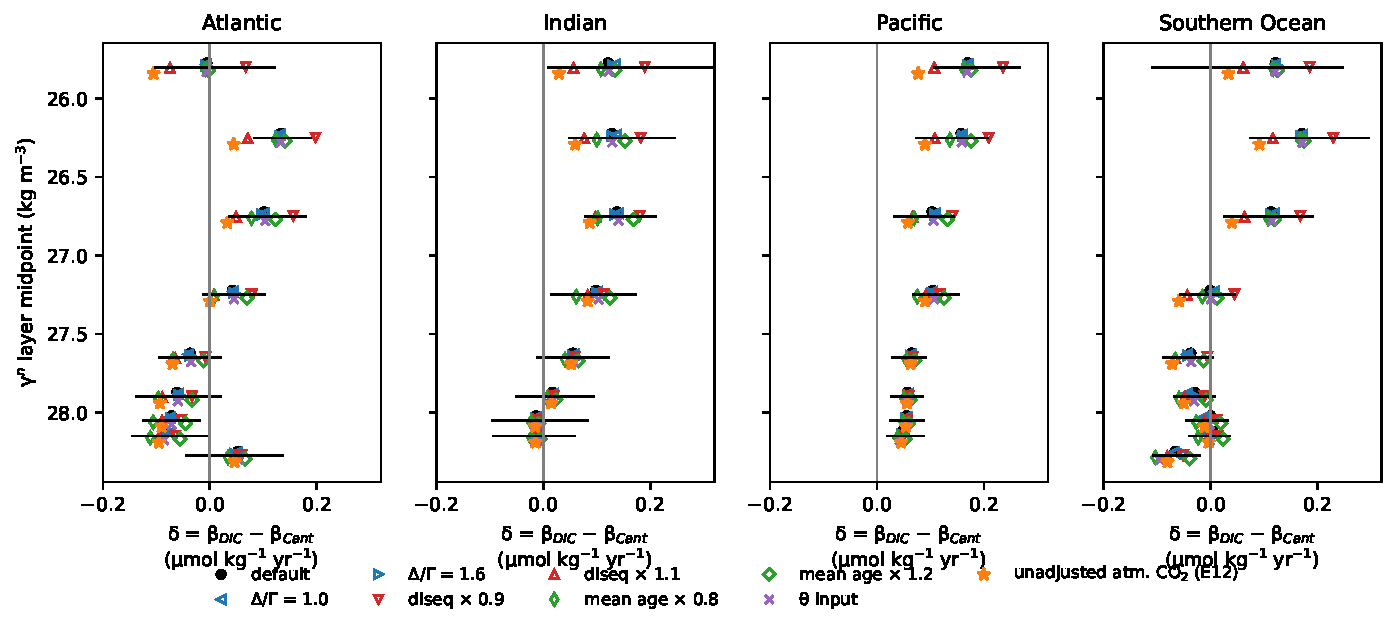
\includegraphics[width=1\linewidth,height=\textheight,keepaspectratio,alt={δ
for TRACE structural variants, from the single-layer estimator with DIC
unchanged. Default with 95 \% interval (black).
Transit-time-distribution shape Δ/Γ = 1.0 and 1.6. Disequilibrium scale
×0.9 and ×1.1. Mean ages ×0.8 and ×1.2. Potential temperature as input.
Unadjusted atmospheric CO2 boundary condition (orange stars; E12, post
hoc).}]{figures/fig9_trace_sensitivity.pdf}
\caption{δ for TRACE structural variants, from the single-layer
estimator with DIC unchanged. Default with 95 \% interval (black).
Transit-time-distribution shape Δ/Γ = 1.0 and 1.6. Disequilibrium scale
×0.9 and ×1.1. Mean ages ×0.8 and ×1.2. Potential temperature as input.
Unadjusted atmospheric CO\textsubscript{2} boundary condition (orange
stars; E12, post hoc).}
\end{figure}

\begin{itemize}
\tightlist
\item
  \textbf{TTD shape} (Δ/Γ 1.0--1.6) and \textbf{temperature input}:
  change δ by ≤ 0.015.
\item
  \textbf{Mean ages ±20 \%}: change δ by −0.04 to +0.03.
\item
  \textbf{Air--sea disequilibrium scale ±10 \%}: changes upper-layer δ
  by ±0.03--0.07, the dominant knob.
\end{itemize}

The excess persists in every variant in the Pacific and in one or more
upper layers of each other basin.

TRACE's built-in surface boundary condition grows at 0.88 times the
atmospheric rate over 1972--2021: it encodes a damped surface-ocean
response. Replacing it with the atmospheric record raises TRACE rates by
9--10 \% (E12, post hoc). This lowers the pooled upper-ocean ratio to R
= 1.06 {[}1.01, 1.10{]} and the differential factor to m = 0.075
{[}0.014, 0.12{]}. An undamped boundary condition therefore accounts for
about 60 \% of the excess. A residual of 6--8 \% remains, and its
interval narrowly excludes zero. The prediction logged before this test
(R within 0.95--1.05) was not met. In the Earth-system-model test
(§4.9), the same substitution removes most of the model-world shortfall.

\subsection{The excess does not depend on AOU conditioning, except in
the Pacific
thermocline}\label{the-excess-does-not-depend-on-aou-conditioning-except-in-the-pacific-thermocline}

C*, which removes soft-tissue and carbonate-pump contributions using
measured phosphate and alkalinity instead of AOU, gives an upper-ocean
excess with CI \textgreater{} 0 in 9 of 12 layers. The AOU estimator
gives the same count on the same rows (E08; Fig. 6).

\begin{figure}
\centering
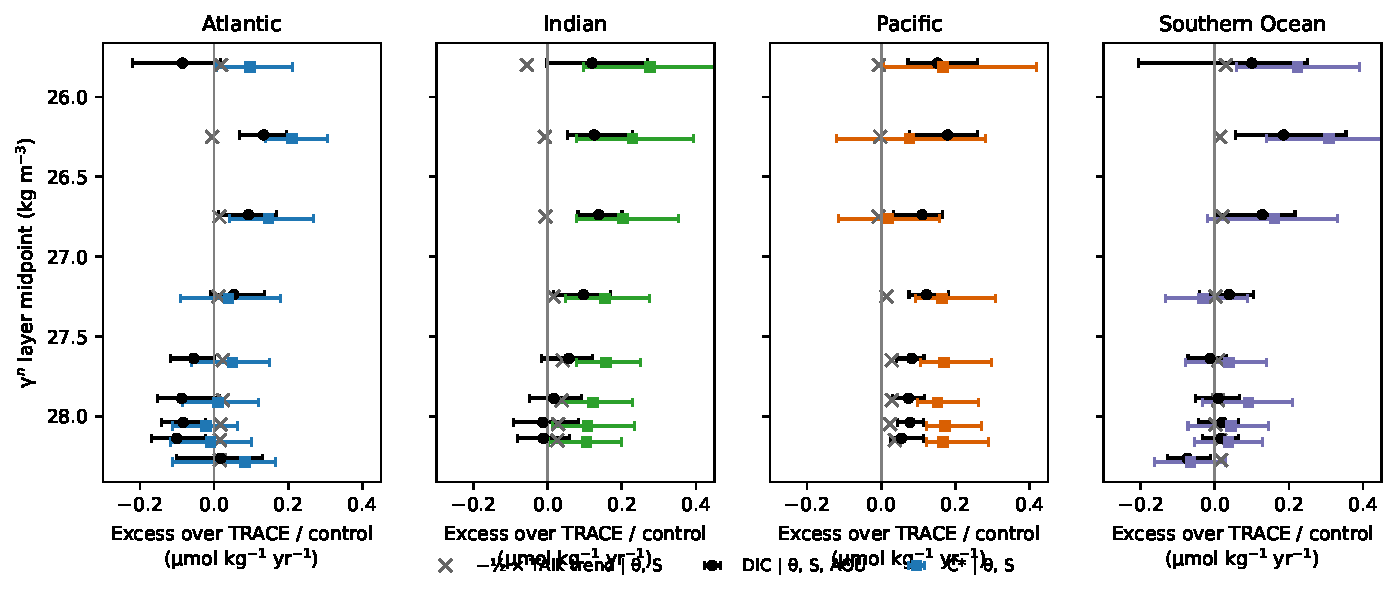
\includegraphics[width=1\linewidth,height=\textheight,keepaspectratio,alt={Sensitivity
to the remineralisation correction, on samples with quality-controlled
PO4 and TAlk. Excess of DIC over TRACE conditioned on θ, S and AOU
(black). Excess of the pump-corrected tracer C* conditioned on θ and S
(coloured). −½ × the TAlk trend at fixed θ, S (crosses): the alkalinity
contribution to C*. Its negative deep values indicate TAlk measurement
drift.}]{figures/fig11_cstar_controls.pdf}
\caption{Sensitivity to the remineralisation correction, on samples with
quality-controlled PO\textsubscript{4} and TAlk. Excess of DIC over
TRACE conditioned on θ, S and AOU (black). Excess of the pump-corrected
tracer C* conditioned on θ and S (coloured). −½ × the TAlk trend at
fixed θ, S (crosses): the alkalinity contribution to C*. Its negative
deep values indicate TAlk measurement drift.}
\end{figure}

The exception is the Pacific thermocline (γⁿ 26.0--27.0), where AOU at
fixed θ, S rises fastest (+0.16 and +0.43 µmol kg\textsuperscript{−1}
yr\textsuperscript{−1}; deoxygenation). There the C* excess falls to
+0.08 and +0.02 with intervals including zero, so the result in these
layers depends on the choice of remineralisation tracer.

The alkalinity control is informative. TAlk at fixed θ, S
\emph{declines} by 0.05--0.08 µmol kg\textsuperscript{−1}
yr\textsuperscript{−1} in 5 deep Pacific and Indian groups. No ocean
process does this, and it points to TAlk measurement drift (TAlk
reference materials were certified only from 1996). This is a caveat for
C*-based methods in deep water, not for the AOU-based estimator.

\subsection{Two independent eMLR(C*) products show the same upper-ocean
excess}\label{two-independent-emlrc-products-show-the-same-upper-ocean-excess}

At the same samples and periods, and with no regression on our side,
both eMLR(C*) products exceed TRACE in the upper ocean (E10; Fig. 7):

\begin{figure}
\centering
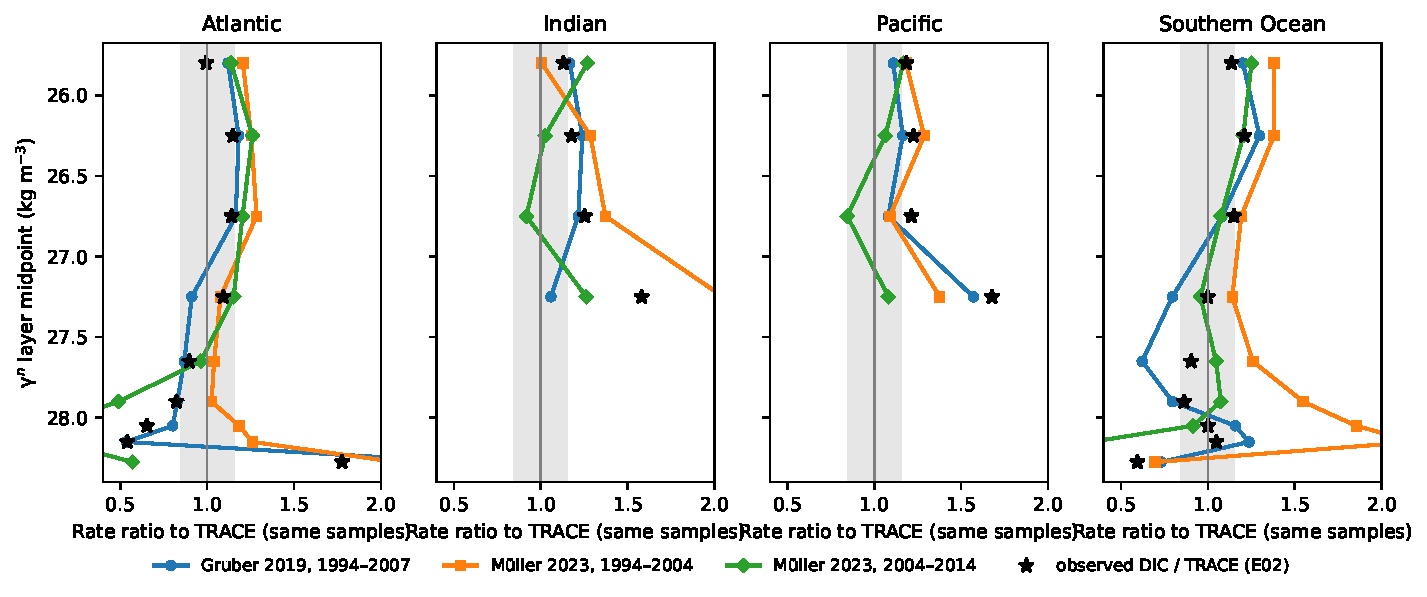
\includegraphics[width=1\linewidth,height=\textheight,keepaspectratio,alt={Ratio
of Cant accumulation rate to TRACE at the same samples and periods, for
layers where the TRACE rate exceeds 0.05 µmol kg−1 yr−1. @Gruber2019,
1994--2007. @Mueller2023, 1994--2004 and 2004--2014 (standard cases).
Observed within-cell DIC (stars). Grey band: ±15 \%. No regression is
involved for the eMLR ratios.}]{figures/fig10_emlr_products.pdf}
\caption{Ratio of C\textsubscript{ant} accumulation rate to TRACE at the
same samples and periods, for layers where the TRACE rate exceeds 0.05
µmol kg\textsuperscript{−1} yr\textsuperscript{−1}. \citet{Gruber2019},
1994--2007. \citet{Mueller2023}, 1994--2004 and 2004--2014 (standard
cases). Observed within-cell DIC (stars). Grey band: ±15 \%. No
regression is involved for the eMLR ratios.}
\end{figure}

{\def\LTcaptype{none} % do not increment counter
\begin{longtable}[]{@{}
  >{\raggedright\arraybackslash}p{(\linewidth - 4\tabcolsep) * \real{0.3333}}
  >{\raggedright\arraybackslash}p{(\linewidth - 4\tabcolsep) * \real{0.3333}}
  >{\raggedright\arraybackslash}p{(\linewidth - 4\tabcolsep) * \real{0.3333}}@{}}
\toprule\noalign{}
\begin{minipage}[b]{\linewidth}\raggedright
Product and period
\end{minipage} & \begin{minipage}[b]{\linewidth}\raggedright
Upper-ocean ratio to TRACE
\end{minipage} & \begin{minipage}[b]{\linewidth}\raggedright
Sensitivity-case range
\end{minipage} \\
\midrule\noalign{}
\endhead
\bottomrule\noalign{}
\endlastfoot
\citet{Gruber2019}, 1994--2007 & 1.13 & 1.06--1.27 \\
\citet{Mueller2023}, 1994--2004 & 1.20 & 1.01--1.25 \\
\citet{Mueller2023}, 2004--2014 & 1.13 & --- \\
\end{longtable}
}

Even the lowest sensitivity case of each product exceeds TRACE. In the
deep Atlantic both products, like observed DIC (R = 0.75), fall below
TRACE: 0.80 (1994--2007) and 0.35 (2004--2014). This is consistent with
reduced deep ventilation and North Atlantic departures from steady state
\citep{Gruber2019, Steinfeldt2024}.

\subsection{A perfect-model test: an Earth system model sampled like
GLODAP}\label{a-perfect-model-test-an-earth-system-model-sampled-like-glodap}

In MRI-ESM2-0 sampled at the GLODAP samples (E13; Fig. 8), anthropogenic
carbon is known exactly, and no GLODAP DIC is involved. The model fields
resemble the observations (correlation with observed θ 0.98, DIC 0.90;
mean DIC bias −26 µmol kg\textsuperscript{−1}).

\begin{figure}
\centering
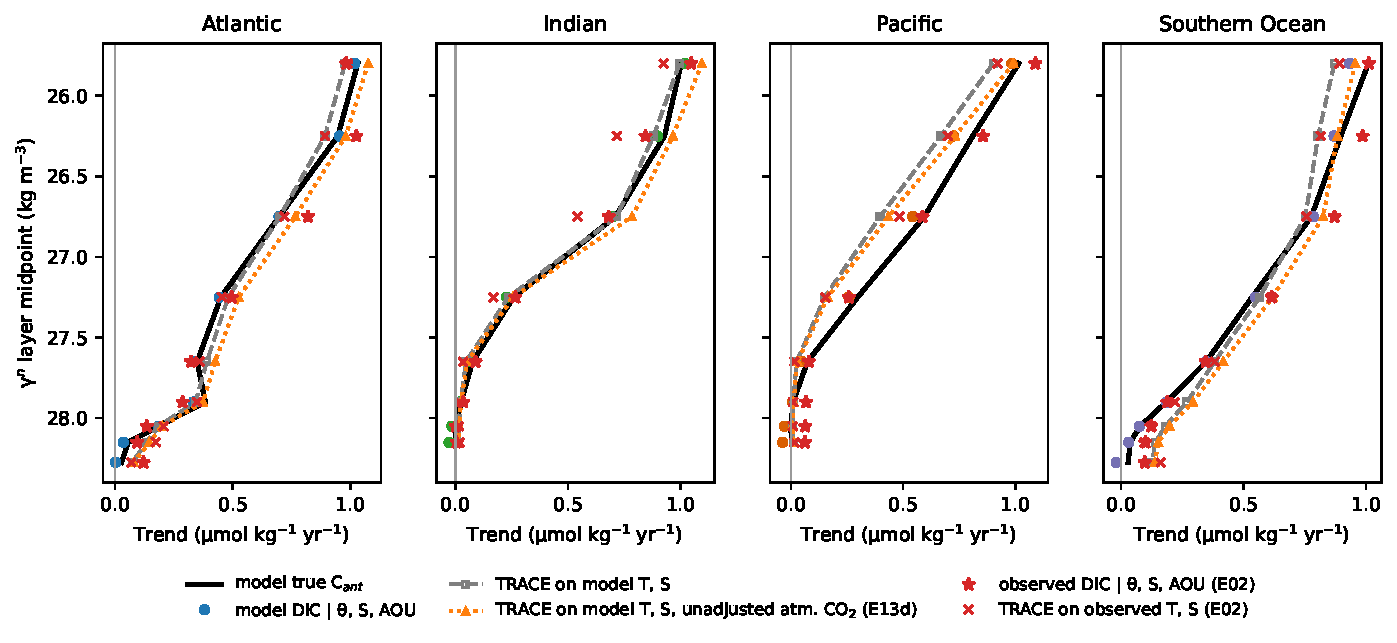
\includegraphics[width=1\linewidth,height=\textheight,keepaspectratio,alt={Perfect-model
test in MRI-ESM2-0 sampled at the GLODAP samples (E13), by basin and
neutral-density layer; within-cell trends at fixed θ, S, AOU. Model true
Cant (DIC − natural DIC; black line). Model DIC (circles): the estimator
applied to model data. TRACE on model T, S, with default (grey squares)
and unadjusted atmospheric (orange triangles, E13d) boundary conditions.
Observed DIC (red stars) and TRACE on observed T, S (red crosses), from
E02, for reference.}]{figures/fig12_perfect_model.pdf}
\caption{Perfect-model test in MRI-ESM2-0 sampled at the GLODAP samples
(E13), by basin and neutral-density layer; within-cell trends at fixed
θ, S, AOU. Model true C\textsubscript{ant} (DIC − natural DIC; black
line). Model DIC (circles): the estimator applied to model data. TRACE
on model T, S, with default (grey squares) and unadjusted atmospheric
(orange triangles, E13d) boundary conditions. Observed DIC (red stars)
and TRACE on observed T, S (red crosses), from E02, for reference.}
\end{figure}

\textbf{The estimators recover the model's true C\textsubscript{ant}
rate.} Upper ocean, pooled:

\begin{itemize}
\tightlist
\item
  single-layer:
  β\textsubscript{DIC}/β\textsubscript{Cant}\textsuperscript{true} =
  0.97 {[}0.95, 0.98{]}, δ = −0.027;
\item
  drift-immune: m = −0.01 {[}−0.04, 0.02{]}.
\end{itemize}

This meets the pre-registered criterion (R within 0.95--1.05,
\textbar δ\textbar{} ≤ 0.03). The only basin-level bias is in the
Pacific (R = 0.95; m = −0.06 {[}−0.11, −0.03{]}), consistent with
circulation-driven AOU change in the thermocline \citep{Sabine2008}. It
biases the estimate toward \emph{less} excess, so the observed Pacific
excess, if anything, is understated. In deep layers, model DIC at fixed
properties rises 0.02 µmol kg\textsuperscript{−1} yr\textsuperscript{−1}
less than C\textsubscript{ant}\textsuperscript{true}: a measure of
non-anthropogenic change in the model.

\textbf{TRACE underestimates the model's own upper-ocean
C\textsubscript{ant} accumulation.} With TRACE run on model T and S:

{\def\LTcaptype{none} % do not increment counter
\begin{longtable}[]{@{}
  >{\raggedright\arraybackslash}p{(\linewidth - 4\tabcolsep) * \real{0.3333}}
  >{\raggedright\arraybackslash}p{(\linewidth - 4\tabcolsep) * \real{0.3333}}
  >{\raggedright\arraybackslash}p{(\linewidth - 4\tabcolsep) * \real{0.3333}}@{}}
\toprule\noalign{}
\begin{minipage}[b]{\linewidth}\raggedright
\end{minipage} & \begin{minipage}[b]{\linewidth}\raggedright
Upper ocean (pooled)
\end{minipage} & \begin{minipage}[b]{\linewidth}\raggedright
Differential
\end{minipage} \\
\midrule\noalign{}
\endhead
\bottomrule\noalign{}
\endlastfoot
C\textsubscript{ant}\textsuperscript{true} / TRACE & 1.12 {[}1.10,
1.14{]} & m = 0.125 {[}0.10, 0.15{]} \\
Model DIC / TRACE (analogue of the observed comparison) & 1.08 {[}1.06,
1.10{]} & m = 0.12 {[}0.08, 0.15{]} \\
\end{longtable}
}

The sign and roughly two thirds of the observed size are reproduced
without GLODAP DIC. Restricting the samples to 1972--2014 (no scenario
years) gives the same result:
C\textsubscript{ant}\textsuperscript{true}/TRACE = 1.117 {[}1.098,
1.144{]}, m = 0.13. The basin pattern is not: the model shortfall is
concentrated in the Pacific (1.18) and Southern Ocean (1.06), with only
1.04 in the Atlantic and 1.01 in the Indian Ocean, whereas the
observations show 16--20 \% in all basins. In deep layers, TRACE
\emph{over}estimates the model (0.76), as expected because CMIP-class
models ventilate the deep ocean more slowly than the real ocean on which
TRACE's ages are trained.

\textbf{The boundary condition accounts for most of the model-world
shortfall (E13d, post hoc).} With TRACE's unadjusted atmospheric
trajectory, the upper-ocean ratio falls to 1.016 {[}1.004, 1.036{]} and
m to 0.024 {[}0.003, 0.050{]}, meeting the logged expectation (R within
0.95--1.05). By basin it overshoots in the Atlantic (0.94) and Indian
(0.92) Oceans and leaves +8 \% in the Pacific.

TRACE's ages describe the real ocean, not the model's circulation, so
this is not a clean test of TRACE. It does show three things:

\begin{itemize}
\tightlist
\item
  in a model whose surface C\textsubscript{ant} follows its own air--sea
  exchange, the upper ocean accumulates C\textsubscript{ant} 10--12 \%
  faster than TRACE with its damped boundary condition implies;
\item
  most of that gap is the boundary condition;
\item
  the estimators themselves introduce no positive bias.
\end{itemize}

\subsection{Time shape and data
quality}\label{time-shape-and-data-quality}

With a knot at 2000, the upper-ocean excess appears in the post-2000
slopes, when DIC reference materials were in routine use. It is
significant in Atlantic γⁿ 26.0--27.0, the Pacific surface layer and
Southern Ocean γⁿ 26.0--26.5. Pre-2000 slopes are too uncertain to test
for a change (E09).

Strict versus relaxed QC changes deep-layer trends by ≤ 0.023 µmol
kg\textsuperscript{−1} yr\textsuperscript{−1}, so H4 (QC sensitivity) is
not supported.

\subsection{Consequences for static empirical DIC
models}\label{consequences-for-static-empirical-dic-models}

Static S--T--AOU regressions trained before 2015 underpredict later DIC
by 4--11 µmol kg\textsuperscript{−1} in every basin. A linear time term
removes ≥ 70 \% of this bias in 36 of 40 cases (median 83 \%) (Fig. 9).
Model rankings depend on the validation design. With a correct
cruise-cluster bootstrap, the rank-1, rank-2 and full-quadratic forms
are equivalent within ±4 µmol kg\textsuperscript{−1} in all 48
comparisons.

\begin{figure}
\centering
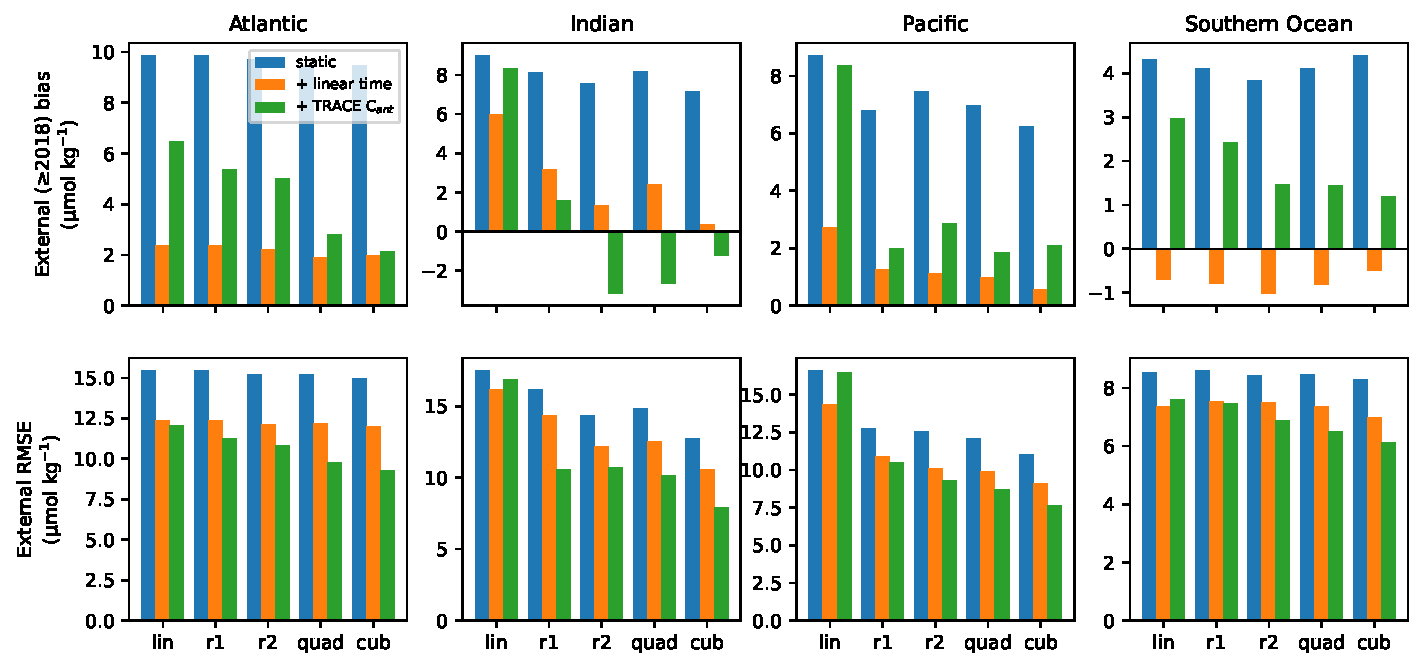
\includegraphics[width=1\linewidth,height=\textheight,keepaspectratio,alt={Static
empirical DIC models trained on years \textless{} 2015 and evaluated on
years ≥ 2018 (strict QC). Top: mean bias (µmol kg−1). Bottom: RMSE (µmol
kg−1). Bars compare static models, models with a linear time term, and
models with a TRACE Cant covariate.}]{figures/fig5_h3_holdout_bias.pdf}
\caption{Static empirical DIC models trained on years \textless{} 2015
and evaluated on years ≥ 2018 (strict QC). Top: mean bias (µmol
kg\textsuperscript{−1}). Bottom: RMSE (µmol kg\textsuperscript{−1}).
Bars compare static models, models with a linear time term, and models
with a TRACE C\textsubscript{ant} covariate.}
\end{figure}

\section{Discussion}\label{discussion}

\textbf{A robust, quantified discrepancy.} Five DIC-based estimates of
upper-ocean carbon accumulation exceed TRACE by 13--20 \% at the same
samples:

\begin{itemize}
\tightlist
\item
  the single-layer trend (1.16);
\item
  the drift-immune differential trend (1 + m = 1.18);
\item
  two eMLR(C*) products over three periods (1.13, 1.20, 1.13).
\end{itemize}

Our estimators use AOU or C* conditioning within fixed locations.
eMLR(C*) uses period-wise multiple linear regressions on mapped
climatologies. The estimates are therefore methodologically distinct,
but not statistically independent: all draw on GLODAP DIC.

An Earth system model sampled at the same points provides evidence that
does not use GLODAP DIC (§4.9). There the estimators are unbiased (m =
−0.01), and TRACE falls short of the model's exact C\textsubscript{ant}
accumulation by a similar factor (m = 0.125).

The new design element makes the most common objection untenable: that
the excess is a slow calibration drift. Additive cruise offsets,
including drifting ones, cannot produce it. A uniform scale
(proportional) drift would bias the single-layer and the differential
estimates in opposite directions, yet both are positive. With a
reference only a few hundred metres deeper, about 70 \% of the excess
remains (E16). What would still be needed is a measurement artefact
within cruises that depends on depth in a more complex way, or a real
excess in the reference layers. The magnitude, about 18 \% of the TRACE
rate, sits at the edge of TRACE's stated 1σ uncertainty of 15 \%. Our
result can therefore be read as an observational constraint on TRACE's
rate scale (1.18 {[}1.11, 1.23{]} relative to the deep ocean), rather
than a refutation of the TTD approach.

\textbf{Candidate explanations, ranked by evidence.}

\begin{enumerate}
\def\labelenumi{\arabic{enumi}.}
\tightlist
\item
  \emph{Surface boundary condition / air--sea disequilibrium.} The
  disequilibrium scale is TRACE's most influential knob. Replacing the
  damped surface trajectory by the atmospheric one removes about 60 \%
  of the observed excess and most of the model-world shortfall (§4.9).
  Multi-decadal time series in the subtropical gyres (BATS, HOT, ESTOC)
  report surface-ocean pCO\textsubscript{2} rising at 1.7--1.9 µatm
  yr\textsuperscript{−1}, similar to the atmospheric increase, with a
  roughly constant air--sea ΔpCO\textsubscript{2} \citep[Table
  2]{Bates2014}. This favours a less damped boundary condition there. At
  higher-latitude sites (Iceland Sea, Munida), surface
  pCO\textsubscript{2} rose more slowly (≈1.3 µatm
  yr\textsuperscript{−1}), and in formation regions with short surface
  residence times real disequilibrium is expected. The Southern Ocean
  intermediate layers, which lie below the proportional line, are
  consistent with that.
\item
  \emph{Ventilation ages in intermediate waters.} Excess relative to the
  TRACE rate is largest in Atlantic and Indo-Pacific intermediate layers
  (γⁿ 27.0--27.5). Ages that are too old there, or mixing not captured
  by a single inverse-Gaussian TTD, would produce this; younger ages
  (×0.8) reduce it.
\item
  \emph{Natural (non-C\textsubscript{ant}) DIC change at fixed
  properties.} This cannot be excluded. In the Pacific thermocline, the
  excess depends on the remineralisation tracer, so part of it there may
  be respiration change associated with deoxygenation that AOU and
  phosphate partition differently. Elsewhere, a natural DIC \emph{gain}
  would conflict with the net natural carbon \emph{loss} inferred by
  \citet{Mueller2023}.
\end{enumerate}

\textbf{Deep ocean.} The deep Atlantic falls 25--35 \% below TRACE in
observed DIC and in both eMLR(C*) products. This matches reported
weakening of North Atlantic ventilation and non-steady-state behaviour
\citep{Gruber2019, Steinfeldt2024}, and strengthens to about 30--50 \%
with the undamped boundary condition. Two caveats apply:

\begin{itemize}
\tightlist
\item
  The deep Pacific excess (+0.05 µmol kg\textsuperscript{−1}
  yr\textsuperscript{−1}, about 2 µmol kg\textsuperscript{−1} over the
  record) is below GLODAP's adjustment threshold and is the most likely
  signature of residual offsets.
\item
  The opposite signs in the deep Atlantic and Pacific are why the
  drift-immune design matters for the upper ocean.
\end{itemize}

\textbf{Implications.}

\begin{itemize}
\tightlist
\item
  TTD-based C\textsubscript{ant} products, including TRACE, are used to
  normalise DIC to reference years (ESPER; mapped GLODAP) and to
  estimate inventories. A 15--20 \% low bias in upper-ocean
  \emph{rates}, if confirmed, would propagate into ocean-acidification
  and sink estimates that use them.
\item
  The diagnostic itself is reusable: a cruise-fixed-effects,
  sample-matched trend comparison can test any interior
  C\textsubscript{ant} product, model or data-based, against
  observations without mapping.
\item
  For empirical DIC models, temporal holdouts are dominated by the
  anthropogenic trend, and functional-form conclusions drawn from them
  are not meaningful without modelling it.
\end{itemize}

\section{Limitations}\label{limitations}

\begin{itemize}
\tightlist
\item
  \textbf{Independence.} All five DIC-based estimates use GLODAP DIC.
  Uniform scale drift is excluded (E16b), and most of the excess remains
  against a near reference (E16). A more complex depth-dependent
  artefact within cruises cannot be excluded, and the near-reference
  estimate is about 30 \% lower. The Earth-system-model test is
  independent of GLODAP DIC, but:

  \begin{itemize}
  \tightlist
  \item
    it is a single model and member. A second model (NorESM2-LM,
    1972--2014) was pre-registered and its sampling code is in place,
    but the run could not be completed because of data-transfer limits
    (\textasciitilde45 GB);
  \item
    the model's basin pattern differs from the observed one;
  \item
    TRACE's ages are not the model's ages;
  \item
    1.8 \% of samples (warm, salty thermocline waters) return no TRACE
    value for model T, S and are excluded from E13.
  \end{itemize}
\item
  \textbf{Reference-layer assumption.} Δδ is relative to the deep
  layers. If deep layers truly accumulate less than TRACE (Atlantic) or
  more (Pacific), Δδ over- or underestimates the absolute excess. We
  bracket it with δ and Δδ. Restricting the reference to γⁿ 27.8--28.0
  or \textgreater{} 28.0 changes m by ≤ 0.02.
\item
  \textbf{Post hoc elements.} E11 (proportional form), E12 and E13d
  (boundary condition) were formulated after seeing the results.
\item
  \textbf{Single linear trend per layer.} Rates under transient steady
  state increase in time. Sample matching makes the comparison
  like-for-like, but R is period-weighted; the piecewise analysis cannot
  resolve era differences before 2000.
\item
  \textbf{Interval coverage.} About 91 \% (single-layer) under large
  random cruise offsets; 93--100 \% for the differential estimator in
  synthetic tests.
\item
  \textbf{Conditioning.} AOU is not true oxygen utilisation in Southern
  Ocean source waters. C* is compromised at depth by TAlk drift.
\item
  \textbf{Coverage.} Analysis is restricted to repeat-sampled cells;
  marginal seas and the Arctic are excluded; the Indian Ocean has 29--36
  cruises per layer.
\item
  \textbf{Not causal.} Attribution among boundary condition, ventilation
  ages and natural carbon change is inferential.
\end{itemize}

\section{Conclusions}\label{conclusions}

\begin{enumerate}
\def\labelenumi{\arabic{enumi}.}
\tightlist
\item
  At fixed water properties and within fixed locations, GLODAP DIC rose
  by about 1 µmol kg\textsuperscript{−1} yr\textsuperscript{−1} in light
  layers, decreasing with density and water-mass age.
\item
  In the upper ocean (γⁿ ≤ 27.0), observed DIC accumulates 16 \% {[}11,
  21 \%{]} faster than TRACE predicts at the same samples, and 18 \%
  {[}11, 23 \%{]} relative to the deep ocean when all cruise-level
  offsets are removed. The excess is similar in all four basins,
  survives every TRACE structural variant in most layers, and is matched
  by two eMLR(C*) products (13--20 \%).
\item
  About 60 \% of the excess is equivalent to replacing TRACE's damped
  surface CO\textsubscript{2} boundary condition with the atmospheric
  record. The remainder points to intermediate-water ventilation ages or
  natural carbon change.
\item
  In an Earth system model sampled like GLODAP, the estimators recover
  the exact C\textsubscript{ant} rate (no positive bias). TRACE falls 12
  \% short of the model's upper-ocean accumulation, mostly because of
  the same boundary condition. This is support that does not rely on
  GLODAP DIC, though with a different basin pattern.
\item
  Deep Atlantic carbon accumulates 25--35 \% below the steady-state
  tracer expectation in observations and eMLR(C*), consistent with
  non-steady ventilation.
\item
  Static DIC regressions are confounded by this signal, and their
  temporal-validation rankings are not interpretable without modelling
  it.
\end{enumerate}

\section*{Open Research}\label{open-research}
\addcontentsline{toc}{section}{Open Research}

\textbf{Data.}

\begin{itemize}
\tightlist
\item
  GLODAPv2.2023: NOAA NCEI accession 0283442.
\item
  \citet{Gruber2019} ΔC\textsubscript{ant}: NCEI 0186034,
  doi:10.25921/wdn2-pt10.
\item
  \citet{Mueller2023} ΔC\textsubscript{ant}: NCEI 0279447.
\item
  TRACE-Python v1.1.2: doi:10.5281/zenodo.17822675.
\item
  MRI-ESM2-0 CMIP6 output (historical, ssp585; r1i2p1f1; gr; v20200303):
  ESGF, via the Pangeo CMIP6 Google Cloud catalogue.
\end{itemize}

Derived datasets are rebuilt by
\texttt{research/preprocessing/build\_dataset.py} (checksum-verified).

\textbf{Software.} All code is in \texttt{research/} (branch
\texttt{research/dev}), and every result has a logged command. Unit
tests are in \texttt{tests/test\_research\_estimators.py}.


\bibliographystyle{plainnat}
\bibliography{references}
\end{document}
